\documentclass[aip,jcp,reprint,amsmath,amssymb]{revtex4-1}

\usepackage{graphicx}% Include figure files
\usepackage{dcolumn}% Align table columns on decimal point
\usepackage{bm}% bold math
\usepackage{amsmath}% bold math
\usepackage{siunitx}% si units
\usepackage{color}
\usepackage{graphicx}
%\usepackage{algorithmic}
\usepackage{algorithm}
\usepackage{algpseudocode}
%\usepackage[normalem]{ulem}
%\nofiles

%\bibliographystyle{achemso}
%\bibliographystyle{naturemag}
%\bibliographystyle{abbrv}

\begin{document}

\renewcommand{\thefigure}{S\arabic{figure}}

\title{
Supplementary Material: \\
Compact orbitals enable low-cost linear-scaling \emph{ab initio} molecular dynamics for weakly-interacting systems
}

\author{Hayden Scheiber}
\email{scheiber@chem.ubc.ca}
\affiliation{Department of Chemistry, McGill University, 801 Sherbrooke St. West, Montreal, QC~H3A~0B8, Canada}
\author{Yifei Shi}
\affiliation{Department of Chemistry, McGill University, 801 Sherbrooke St. West, Montreal, QC~H3A~0B8, Canada}
\author{Rustam Z. Khaliullin}
\email{rustam.khaliullin@mcgill.ca}
\affiliation{Department of Chemistry, McGill University, 801 Sherbrooke St. West, Montreal, QC~H3A~0B8, Canada}

\maketitle
%\date{\today}

\subsection{Algorithms}

The pseudocode for the new \emph{ab initio} molecular dynamics (AIMD) method is shown in Figure~\ref{fig:ricci}. As described in the main text, the algorithm represents the Ricci-Ciccotti integrator~\cite{Ricci2003} modified (Lines~\ref{line:delta1} and \ref{line:delta2}) to take into account the imperfect forces computed using a constrained density functional theory (DFT) based on absolutely localized molecular orbitals (ALMOs) (Figure~\ref{fig:force}). 

\begin{figure}
\begin{algorithm}[H]
  \caption{Modified Ricci-Ciccotti integrator}
  \label{alg:ricci}
   \begin{algorithmic}[1]
   	\State Input $t$ \Comment{Time step}
   	\State Input $N$ \Comment{Number of AIMD steps}
   	\State Input $T$ \Comment{Temperature}
   	\State Input $\gamma$ \Comment{Langevin damping coefficient}
   	\State Input $\Delta$ \Comment{Compensation for imperfect forces} \label{line:delta1}
   	\State Input $A$ \Comment{Number of atoms}
	\State $\tau\gets 0$ \Comment{Current time step}
	\State Allocate $\mathbf{r}, \mathbf{p}, \mathbf{f}$ \Comment{Matrices: positions, momenta, forces}
   	\State Input $\mathbf{r}$
	\State $\mathbf{p} \gets \text{Maxwell-Boltzmann}(T)$ \Comment{Generate initial momenta}
	\State $\mathbf{f} \gets \text{ALMO.Force}(\mathbf{r},\tau)$ \Comment{Compute forces (Algorithm~\ref{alg:force})}
	\For{$\tau \gets 1$ to $N$} \Comment{Time loop}
		\For{$i \gets 1$ to $A$} \Comment{Loop over atoms}
			\State $\sigma_i \gets 2 k_B T m_i t (\gamma + \Delta)$  \label{line:delta2}
			\State $\vec{w}_{i} \gets \mathcal{N}(0,\sigma_i)$ \Comment{Vector of random numbers}
			\State $\vec{r}_i \gets \vec{r}_i + \mathrm{e}^{-\gamma t/2} \frac{t}{m_i}\vec{p}_i + \mathrm{e}^{-\gamma t/4} \frac{t}{2 m_i} \left( t \vec{f}_i + \vec{w}_i \right) $
			\State $\vec{p}_i \gets \vec{p}_i + \mathrm{e}^{\gamma t/2} \frac{t}{2} \vec{f}_i$ \Comment{Start updating momenta}
		\EndFor
		\State $\mathbf{f} \gets \text{ALMO.Force}(\mathbf{r},\tau)$ \Comment{Update forces}
		\For{$i \gets 1$ to $A$}
%			\State $\vec{p}_i \gets \mathrm{e}^{-\gamma t} \left( \vec{p}_i + \mathrm{e}^{\gamma t/2} \frac{t}{2} \vec{f}_i \right) + \mathrm{e}^{-\gamma t/2} \vec{w}_i $   \Comment{Update momenta}
			\State $\vec{p}_i \gets \vec{p}_i + \mathrm{e}^{\gamma t/2} \frac{t}{2} \vec{f}_i $
			\State $\vec{p}_i \gets \mathrm{e}^{-\gamma t} \vec{p}_i + \mathrm{e}^{-\gamma t/2} \vec{w}_i $   \Comment{Update momenta}
		\EndFor
	\EndFor
   \end{algorithmic}
\end{algorithm}
\caption{\label{fig:ricci} ALMO AIMD algorithm.}
\end{figure}

\begin{figure}
\begin{algorithm}[H]
  \caption{Force evaluation}
  \label{alg:force}
   \begin{algorithmic}[1]
   	\Procedure{ALMO.Force}{$\mathbf{r}, \tau$}
   	\State Global $\mathbf{S}$ \Comment{Compute AO overlap}
	\State $\mathbf{T}_0 \gets \text{ALMO.Stage1}(\mathbf{r}, \tau)$ \Comment{SCF, Stage 1}
	\State $\mathbf{T}_{R_c} \gets \text{ALMO.Stage2}(\mathbf{r}, \tau, \mathbf{T}_0)$ \Comment{SCF, Stage 2}
	\State $\mathbf{\sigma}, \mathbf{R} \gets \text{Eq.}\ref{eq:dm}(\mathbf{T}_{R_c})$ \Comment{Compute DM}
	\State $\mathbf{F} \gets \text{DFT.BuildKS}(\mathbf{R})$ \Comment{Kohn-Sham matrix}
	\State $\mathbf{W} \gets \mathbf{RFR}$ \Comment{Energy-weighted DM}
	\State $\mathbf{f} \gets \text{DFT.HellmannFeynmanForce}(\mathbf{R},\mathbf{F}) + \text{DFT.PulayForce}(\mathbf{W},\mathbf{S}) $ \Comment{Atomic forces}
	\State $\mathbf{return}$ $\mathbf{f}$
	\EndProcedure
   \end{algorithmic}
\end{algorithm}
\caption{\label{fig:force} ALMO DFT algorithm to compute atomic forces.}
\end{figure}


As described in Refs.~\citenum{a:almo-ls}, ALMO DFT is designed to be computationally efficient for large systems that can be logically partitioned into small fragments---molecules, atoms, ions---not connected to each other by strong covalent bonds. ALMO DFT differs from the conventional DFT only by constraints imposed on electrons: all electrons and AOs in the system are assigned to fragments and each electron is allowed to delocalize only over its own fragment and all neighboring fragments within a pre-defined cutoff radius $R_c$ (Figure~\ref{fig:blocks}A). This restriction imposes the blocked pattern on electron's molecular orbital and the molecular orbital coefficient matrix $\mathbf{T}$ (Figure~\ref{fig:blocks}B).

To simplify equations that involve blocked matrices, the following notation is used. Square brackets $[\mathbf{M}]_{R_c}$ represent an operator that enforces the block structure on matrix $\mathbf{M}$ for a specified $R_c$ (Figure~\ref{fig:blocks}). Once the block structure is imposed any $\text{N}_{\text{AO}} \times \text{N}_{\text{MO}}$ matrix can be represented by two interconvertible formats shown in Figure~\ref{fig:blocks}B. The two formats, denoted by subscript or superscript $R_c$, are necessary to make matrix equations consistent throughout the pseudocode. If $R_c = 0$ the two formats are equivalent. For an $\text{N}_{\text{AO}} \times \text{N}_{\text{AO}}$ matrix, only one blocked format is defined. It is denoted by superscript $R_c$. When used without the superscript, an $\text{N}_{\text{AO}} \times \text{N}_{\text{AO}}$ matrix is not assumed to be blocked, which means that all its blocks are computed. Nevertheless, all algorithms presented here are linear scaling because of the natural sparsity of all $\text{N}_{\text{AO}} \times \text{N}_{\text{AO}}$ matrices. It is important to remind that the square bracket operator and blocked structures in Figure~\ref{fig:blocks} are just a convenient notation. The actual data structures and the implementation of matrix handling subroutines, designed to achieve linear scaling with low computational overhead, are significantly more complex. 

\begin{figure*}
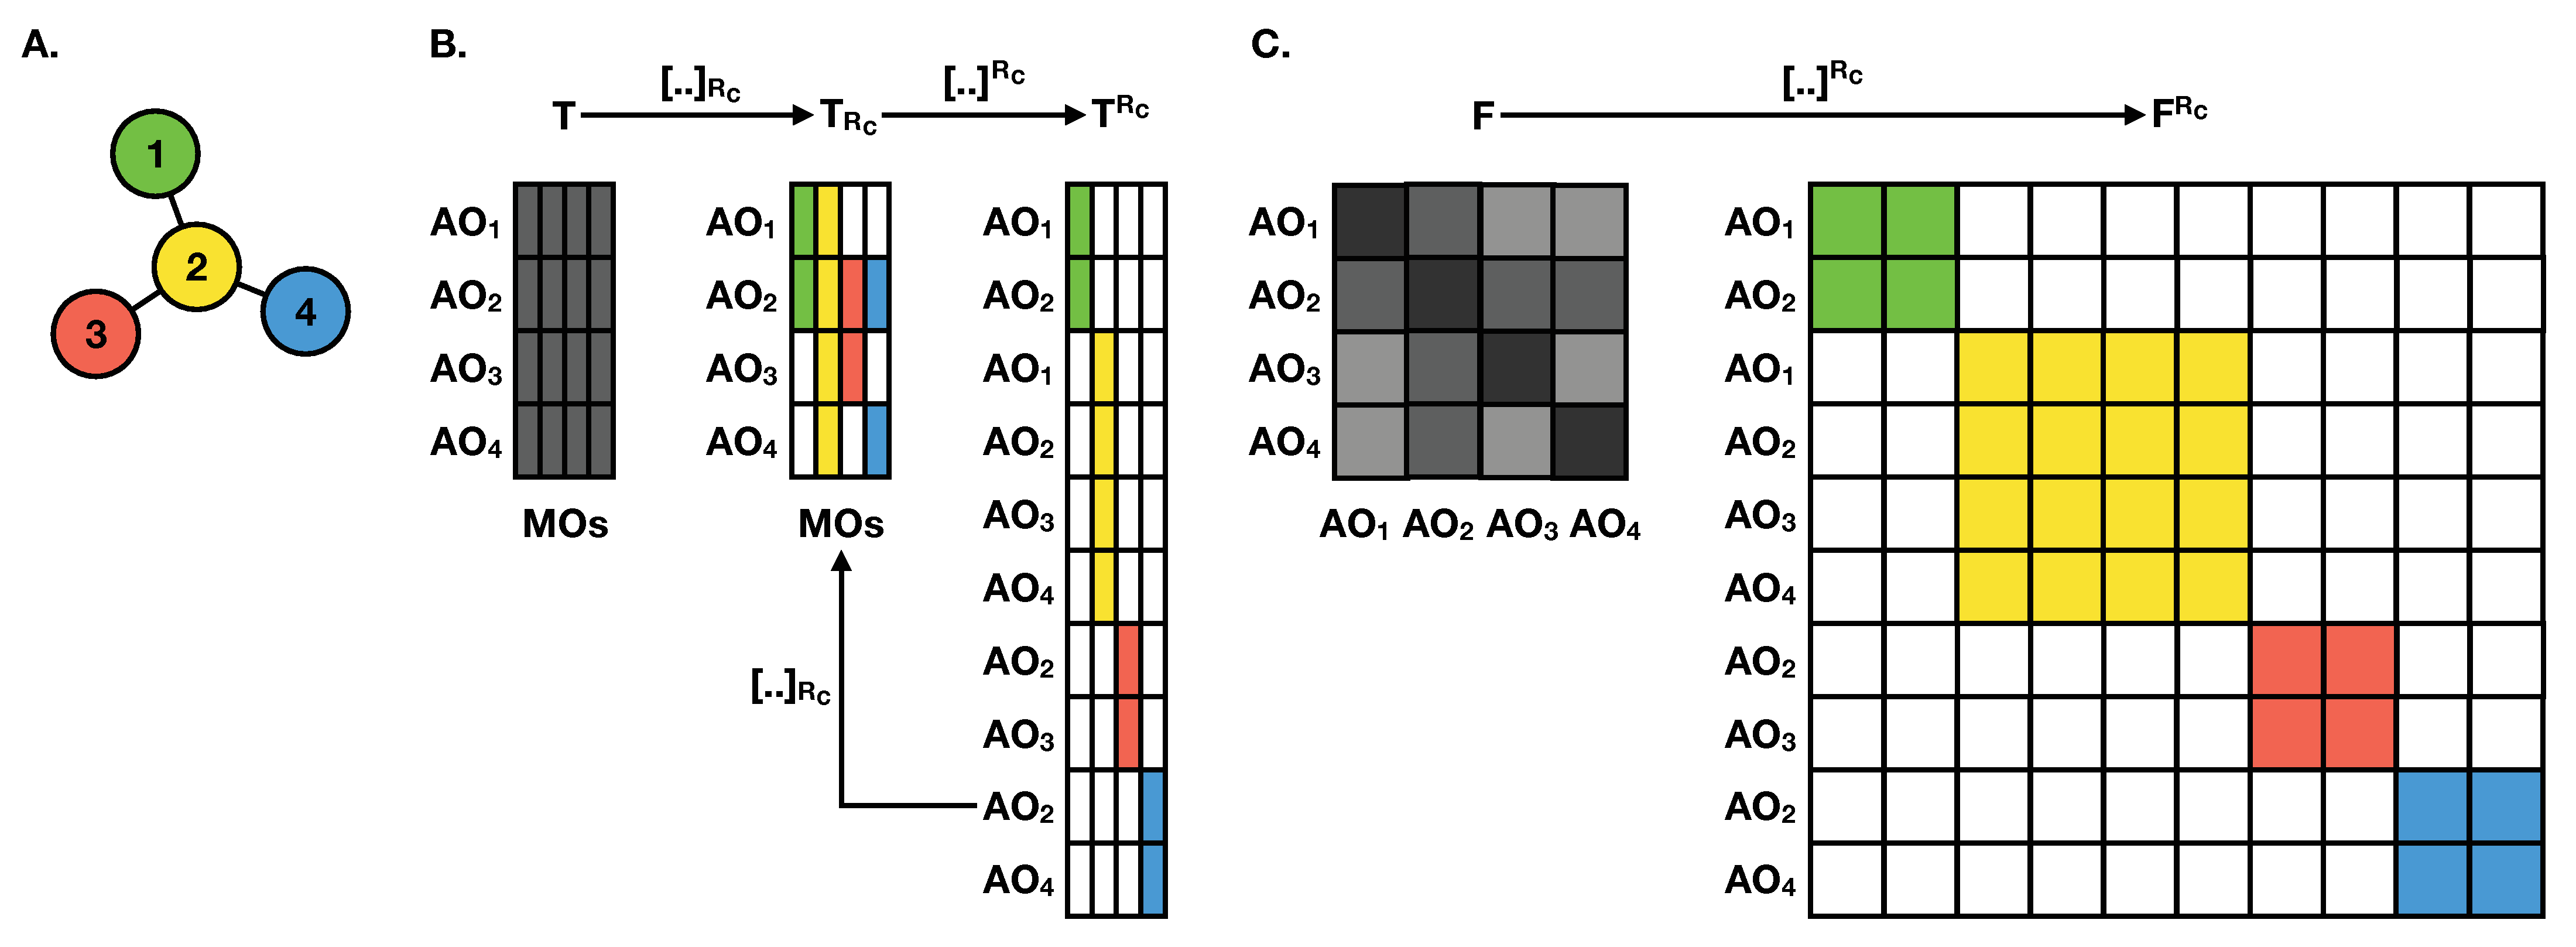
\includegraphics[trim={0cm 0cm 0.1cm 0.1cm},clip,width=17.5cm]{ALMO.eps}
\caption{\label{fig:blocks} Partitioning of a 4-molecule system and the resulting blocked structure imposed on matrices. A. Four molecules are represented by different colors. Solid lines connect neighbors lying within $R_c$ from each other. B. The corresponding blocked structure imposed on an $\text{N}_{\text{AO}} \times \text{N}_{\text{MO}}$ matrix (e.g. molecular orbital coefficient matrix, gradient matrix) and conversion between the two different formats denoted by subscript and superscript $R_c$. White blocks are zero. C. The blocked structure imposed on an $\text{N}_{\text{AO}}\times\text{N}_{\text{AO}}$ matrix (e.g. Kohn-Sham, density matrices).}
\end{figure*}

The algorithms for the force evaluation rely on the following conventions. Functions with names starting with \texttt{ALMO} are written out explicitly. Functions with names starting with \texttt{DFT} are conventional and are not shown. There are two functions that refer to the direct inversion in the iterative subspace (DIIS) method. \texttt{DIIS.push} updates the DIIS matrix and enables \texttt{DIIS.extrapolate} to generate a new variable that, hopefully, minimizes the error. These functions are not written out explicitly. Functions with names starting with \texttt{HISTORY} store and retrieve the contravariant-covariant density matrices from recent AIMD steps. These matrices are necessary to generate a good initial guess for the electronic descriptors in the two self-consistent field (SCF) procedures. The atomic orbital (AO) overlap matrix $\mathbf{S}$ remains constant within one AIMD step and, therefore, is conveniently treated as a global variable visible in all procedures.

As shown in Figure~\ref{fig:force}, ALMO DFT evaluates the final density matrix (DM) in two SCF stages. In both stages, the overlap of ALMOs $\mathbf{\sigma}$ and the density matrix (DM) $\mathbf{R}$ is computed using Eq.~\ref{eq:dm}. Note that these two matrices are naturally sparse, that is, the block structure is not imposed on them.
%
\begin{eqnarray}\label{eq:dm}
\mathbf{\sigma} &=& \mathbf{T}_{R_c}^{\dagger}\mathbf{S} \mathbf{T}_{R_c} \nonumber \\
\mathbf{R} &=& \mathbf{T}_{R_c} \mathbf{\sigma}^{-1} \mathbf{T}_{R_c}^{\dagger}
\end{eqnarray}
%

In the first stage, molecular orbitals are constrained to their fragments and optimized using the DIIS accelerated algorithm in Figure~\ref{fig:almo0}. This algorithm is almost identical to the Stoll algorithm~\cite{a:stoll} of Ref.~\cite{a:khal} and refers to the following equations. The locally projected Hamiltonian~\cite{a:stoll} is computed using Eq.~\ref{eq:lph}. This equation is the same as Eq.~(51) in Ref.~\onlinecite{a:khal}.
%
\begin{eqnarray}\label{eq:lph}
\mathbf{L}_0 &=& [ (\mathbf{1} - \mathbf{SR}) \mathbf{F} (\mathbf{1} - \mathbf{RS}) ]_{0} + \nonumber\\
&+& [ (\mathbf{1} - \mathbf{SR}) \mathbf{FT}_0 \sigma^{-1}]_0 [ \mathbf{T}_0^{\dagger}\mathbf{S} ]_{0} \nonumber\\
&+& [ \mathbf{ST}_0 ]_{0} [ \sigma^{-1}\mathbf{T}_0^{\dagger}\mathbf{F}(\mathbf{1} - \mathbf{RS}) ]_0 + \nonumber\\
&+& [ \mathbf{ST}_0]_0 [ \sigma^{-1}\mathbf{T}_0^{\dagger}\mathbf{FT}_0 \sigma^{-1}]_{0} [ \mathbf{T}_0^{\dagger}\mathbf{S} ]_{0}
\end{eqnarray}
%
The DIIS error in the first stage is computed using Eq.~(\ref{eq:diis-error}) below, which is the same as Eq.~(39) in Ref.~\onlinecite{a:khal}.
%
\begin{eqnarray}\label{eq:diis-error}
\mathbf{G}_0 = [\mathbf{S}]_0 [\mathbf{RF}(\mathbf{RS-1})]_0 - [(\mathbf{SR-1})\mathbf{FR}]_0 [\mathbf{S}]_0
\end{eqnarray}

\begin{figure}
\begin{algorithm}[H]
  \caption{DIIS optimization of block-diagonal ALMOs}
  \label{alg:almo0}
   \begin{algorithmic}[1]
   	\Procedure{ALMO.Stage1}{$\mathbf{r}, \tau$}
	\State Input $\epsilon_{\text{SCF}}$ \Comment{Convergence threshold}
	\State Input $N_{\text{SCF}}$ \Comment{Max SCF iterations}
	\State $\mathbf{K}_0 \gets ([\mathbf{S}]_0)^{-1/2}$ \Comment{Orthogonalization matrix}
	\State $\mathbf{T}_0 \gets \text{ALMO.Guess}(1, 0.0)$ \Comment{MO guess}
	\State $\mathbf{\sigma,R} \gets \text{Eq.\ref{eq:dm}}(\mathbf{T}_0)$ \Comment{Compute DM}
	\State $\mathbf{F} \gets \text{DFT.BuildKS}(\mathbf{R})$ \Comment{Kohn-Sham matrix}

	\State StopSCF $\gets$ False \Comment{Prepare to exit SCF loop}
	\State $i_{\text{SCF}} \gets 0$ \Comment{Iteration counter}
	\Repeat \Comment{SCF loop}
		\State $i_{\text{SCF}} \gets i_{\text{SCF}} + 1$ 
		\State $\mathbf{L}_{0} \gets \text{Eq.}\ref{eq:lph}(\mathbf{F},\mathbf{R},\mathbf{T}_0,\mathbf{\sigma})$ \Comment{Projected KS matrix}
		\State $\mathbf{G}_0 \gets \text{Eq.\ref{eq:diis-error}}(\mathbf{F},\mathbf{R})$ \Comment{DIIS error}
		\State DIIS.push($\mathbf{L}_{0}, \mathbf{G}_{0}$)
		\State $\text{Error}_\text{SCF} \gets \vert\vert \mathbf{G}_0 \vert \vert_{\text{max}}$
		\If{$\text{Error}_\text{SCF} > \epsilon_{\text{SCF}}$}
			\State Converged $\gets$ False
		\Else
			\State Converged $\gets$ True
		\EndIf
		\If{$i_{\text{SCF}} > N_{\text{SCF}}$ \textbf{Or} Converged}
			\State StopSCF $\gets$ True
		\EndIf
		\If{$i_{\text{SCF}}=1$}
			\State StopSCF $\gets$ False \Comment{Do at least one iteration}
		\EndIf
		\If{Not StopSCF}
			\State $\mathbf{L}_{0}\gets$DIIS.extrapolate()
			\State $\mathbf{\tilde{M}}_{0} \gets \mathbf{K}_0 \mathbf{L}_{0} \mathbf{K}_0$ \Comment{KS in orthogonal basis}
			\State $\mathbf{\tilde{C}}_0 \gets \text{Solve}[\mathbf{\tilde{M}}_{0} \mathbf{\tilde{C}}_{0} = \mathbf{\tilde{C}}_{0} \mathbf{e}_{0}] $ \Comment{Eigensystem}
			\State $\mathbf{\tilde{T}}_{0} \gets \text{occ}(\mathbf{\tilde{C}}_{0})$ \Comment{Keep occupied orbitals}
			\State $\mathbf{T}_{0} \gets \mathbf{K}_0 \mathbf{\tilde{T}}_{0}$ \Comment{Into nonorthogonal basis}
			\State $\mathbf{\sigma,R} \gets \text{Eq.\ref{eq:dm}}(\mathbf{T}_0)$ \Comment{Compute DM}
			\State $\mathbf{F} \gets \text{DFT.BuildKS}(\mathbf{R})$ \Comment{Kohn-Sham matrix}
		\EndIf
	\Until{StopSCF}
	\State HISTORY.Stage1.Save($\mathbf{RS}$) \Comment{Needed in \texttt{ALMO.Guess}}
	\State HISTORY.Stage1.Save($\mathbf{T}_0$) \Comment{Needed in \texttt{ALMO.Guess}}
	\State $\mathbf{return}$ $\mathbf{T}_0$
	\EndProcedure
   \end{algorithmic}
\end{algorithm}
\caption{\label{fig:almo0} First stage of ALMO DFT computes block-diagonal orbitals ($R_c=0$) using DIIS accelerator.}
\end{figure}


In the second stage, ALMOs are relaxed to allow delocalization onto the neighboring fragments within localization radius $R_{c}$. In this stage, ALMOs are completely defined using the block-diagonal reference from the first stage and the delocalization amplitudes $\mathbf{X}_{R_c}$ (Line~\ref{line:almos} in Figure~\ref{fig:almoR}). It is the delocalization amplitudes that serve as the variational degrees of freedom (DOFs) in the optimization SCF procedure. The optimization is based on a preconditioned conjugate gradient algorithm shown in Figure~\ref{fig:almoR} and described in Ref.~\citenum{a:almo-ls}. The preconditioner in the second stage is computed using Eq.~(\ref{eq:prec}) below, which is the same as Eq.~(10) in Ref.~\onlinecite{a:almo-ls}.
%
\begin{eqnarray}\label{eq:prec}
\mathbf{P}^{R_c} =  (\mathbf{I} - \mathbf{M}^{R_c} \mathbf{K}^{R_c}) [\mathbf{S+F}]^{R_c} (\mathbf{I} - \mathbf{K}^{R_c} \mathbf{M}^{R_c})
\end{eqnarray}


\begin{figure}
\begin{algorithm}[H]
  \caption{PCG optimization of ALMOs}
  \label{alg:almoR}
   \begin{algorithmic}[1]
   	\Procedure{ALMO.Stage2}{$\mathbf{r}, \tau, \mathbf{T}_0$}
	\State Input $R_c$ \Comment{Electron localization radius}
	\State Input $\epsilon_{\text{SCF}}$ \Comment{Convergence threshold}
	\State Input $N_{\text{PCG}}$, $N_{\text{Outer}}$ \Comment{Max PCG, outer iterations}
	\State $\mathbf{K}^{R_c} \gets ([\mathbf{S}]^{R_c})^{-1}$ \Comment{Inverted blocked AO overlap}
	\State $\mathbf{\sigma,R} \gets \text{Eq.\ref{eq:dm}}(\mathbf{T}_{0})$ \Comment{DM}
	\State $\mathbf{M}^{R_c} \gets [\mathbf{SRS}]^{R_c}$ \Comment{Blocked covariant projector}
	
	\State $\mathbf{X}_{R_c} \gets \text{ALMO.Guess}(2, R_c, \mathbf{T}_0)$ \Comment{Variational DOFs}

	\State Converged $\gets$ False
	\State StopOuter $\gets$ False \Comment{Flag to exit the outer loop}
	\State $i_{\text{Outer}} \gets 0$ \Comment{Iteration counter}
	\Repeat \Comment{Outer loop restarts PCG}
		\State $i_{\text{Outer}} \gets i_{\text{Outer}} + 1$ 
		\State StopPCG $\gets$ False \Comment{Flag to exit the PCG loop}
		\State $i_{\text{PCG}} \gets 0$ \Comment{Iteration counter}
		\State $\beta \gets 0$ \Comment{Reset conjugation}
		\Repeat \Comment{PCG loop}
			\State $i_{\text{PCG}} \gets i_{\text{PCG}} + 1$ 
			\State $\mathbf{T}_{R_c} \gets \mathbf{T}_{0} + [(\mathbf{I} - \mathbf{K}^{R_c} \mathbf{M}^{R_c}) \mathbf{X}^{R_c}]_{R_c}$ \Comment{ALMO} \label{line:almos}
			\State $\mathbf{\sigma,R} \gets \text{Eq.\ref{eq:dm}}(\mathbf{T}_{R_c})$ \Comment{DM}
			\State $\mathbf{F} \gets \text{DFT.BuildKS}(\mathbf{R})$ \Comment{Kohn-Sham matrix}
			\If{$i_{\text{PCG}}>1$}
				\State $\mathbf{\Gamma}_{R_c} \gets \mathbf{G}_{R_c}$ \Comment{Save old gradient}
			\EndIf 
			\State $\mathbf{G}_{R_c} \gets [ (\mathbf{I} - \mathbf{SR}) \mathbf{FT}_{R_c} \mathbf{\sigma}^{-1}]_{R_c}$ \Comment{Gradient}
			\State $\text{Error}_\text{PCG} \gets \vert\vert \mathbf{G}_{R_c} \vert \vert_{\text{max}}$
			\If{$\text{Error}_\text{PCG} < \epsilon_{\text{SCF}}$}
				\State Converged $\gets$ True
			\EndIf
			\If{$i_{\text{PCG}} > N_{\text{PCG}}$ \textbf{Or} Converged}
				\State StopPCG $\gets$ True
			\EndIf
			\If{$i_{\text{PCG}}=1$ \textbf{And} $i_{\text{Outer}}=1$}
				\State StopPCG $\gets$ False \Comment{Do first iteration}
			\EndIf
			\If{\textbf{Not} StopPCG}
				\If{$i_{\text{PCG}} = 1$}
					\State $\mathbf{P}^{R_c} \gets \text{Eq.\ref{eq:prec}}(\mathbf{F},\mathbf{M}^{R_c},\mathbf{K}^{R_c}) $\Comment{Precon.}
				\Else
					\State $\mathbf{O}_{R_c} \gets \mathbf{D}_{R_c}$ \Comment{Save old direction}
				\EndIf
				\State $\mathbf{D}_{R_c} \gets - [(\mathbf{P}^{R_c})^{-1} \mathbf{G}^{R_c}]_{R_c}$ \Comment{Precon. grad.}
				\If{$i_{\text{PCG}}>1$}
					\State $\beta \gets \text{Tr}(\mathbf{G}^{\dagger}_{R_c} \mathbf{D}_{R_c})/\text{Tr}(\mathbf{\Gamma}^{\dagger}_{R_c}\mathbf{O}_{R_c})$
				\EndIf 
				\State $\mathbf{D}_{R_c} \gets \mathbf{D}_{R_c} + \beta \mathbf{O}_{R_c}$ \Comment{Search direction}
				\State $\alpha \gets \text{LineSearch}(\mathbf{D}_{R_c})$ \Comment{Step size}
				\State $\mathbf{X}_{R_c} \gets \mathbf{X}_{R_c} + \alpha \mathbf{D}_{R_c}$ \Comment{Update DOFs}
			\EndIf
		\Until{StopPCG} 
		\If{$i_{\text{Outer}} > N_{\text{Outer}}$ \textbf{Or} Converged}
			\State StopOuter $\gets$ True
		\EndIf
	\Until{StopOuter}
	\State HISTORY.Stage2.Save($\mathbf{RS}$) \Comment{Needed in \texttt{ALMO.Guess}}
	\State $\mathbf{return}$ $\mathbf{T}_{R_c}$
	\EndProcedure
   \end{algorithmic}
\end{algorithm}
\caption{\label{fig:almoR} Second stage of ALMO DFT computes orbitals localized on molecules and their neighbors ($R_c$ is finite). The SCF procedure is based on the preconditioned conjugate gradient (PCG) method.}
\end{figure}

The efficiency of both SCF stages is greatly improved by the availability of a good initial guess for the localized electronic descriptors. The initial guess is generated using an algorithm (Figure~\ref{fig:guess}) inspired by the always stable predictor-corrector method of Kolafa~\cite{Kolafa2003}.

\begin{figure}
\begin{algorithm}[H]
  \caption{Initial guess}
  \label{alg:guess}
   \begin{algorithmic}[1]
   	\Procedure{ALMO.Guess}{Stage, $R_c$, optional $\mathbf{T}_{0}$}

	\State $N \gets \text{HISTORY.AccumulatedLength()}$ \Comment{Max 3--5}

	\If{$N = 0$} \Comment{Generate new guess}

		\If{Stage = 1}
			\State $\mathbf{T}_{R_c} \gets \text{Random()}$ %[\text{DFT.SumOfAtomicDensities}]_0
			\State $\mathbf{T}_{R_c} \gets \mathbf{T}_{Rc} ([\mathbf{T}_{Rc}^{\dagger}\mathbf{S}\mathbf{T}_{Rc}]_0)^{-1/2}$ \Comment{Orthogonalize within blocks to preserve locality}
		\Else
			\State $\mathbf{T}_{R_c} \gets 0 $
		\EndIf

	\Else \Comment{Extrapolate}
	
		\State Allocate $\mathbf{RS}(N)$ \Comment{Array of contravariant-covariant DMs from previous AIMD steps, 1st element of the array is the most recent}	
		\If{Stage = 1}
			\State $\mathbf{RS} \gets \text{HISTORY.Stage1.Load()}$ %\Comment{Converged DMs from SCF Stage1}
		\Else
			\State $\mathbf{RS} \gets \text{HISTORY.Stage2.Load()}$ %\Comment{Converged DMs from SCF Stage2}
		\EndIf
		\State $\mathbf{T}_{0}(1) \gets \text{HISTORY.Stage1.Load()}$ \Comment{Converged block-diagonal ALMOs from the previous AIMD step}
		\State $\mathbf{T}_{R_c} \gets 0$
		
		\For{	$m \gets 1, N$}
			\State $\alpha \gets (-1)^{m+1} m \binom{2N}{ N-m} / \binom{2N-2}{N-1}$ 
			\State $\mathbf{T}_{R_c} \gets \mathbf{T}_{R_c} + \alpha [\mathbf{RS}(m) \mathbf{T}_{0}(1)]_{R_c} $ 
			%\State $\mathbf{E}_{R_c} \gets [\mathbf{R}(m) \mathbf{S}(m) \mathbf{T}_{0}(1)]_{R_c}$
			%\State $\mathbf{E}_{R_c} \gets \mathbf{E}_{Rc} ([\mathbf{E}_{Rc}^{\dagger}\mathbf{S}\mathbf{E}_{Rc}]_0)^{-1/2}$
			%\State $\mathbf{T}_{R_c} \gets \mathbf{T}_{R_c} + \frac{\alpha}{N} \mathbf{E}_{Rc}$
		\EndFor
		\State $\mathbf{T}_{R_c} \gets \mathbf{T}_{Rc} ([\mathbf{T}_{Rc}^{\dagger}\mathbf{S}\mathbf{T}_{Rc}]_0)^{-1/2}$ \Comment{Orthogonalize within blocks to preserve locality}
		
		\If{ Stage = 2}
			\State $\mathbf{T}_{R_c} \gets \mathbf{T}_{R_c}  - \mathbf{T}_{0}$
		\EndIf

	\EndIf

	\State $\mathbf{return}$ $\mathbf{T}_{R_c}$
	\EndProcedure
   \end{algorithmic}
\end{algorithm}
\caption{\label{fig:guess} Initial guess for the localized electronic descriptors. The algorithm is inspired by always stable predictor-corrector method of Kolafa~\cite{Kolafa2003}.}
\end{figure}

\subsection{Dependence of the forces on the electron localization radius}

The ALMO forces converge to the reference forces as the electron localization radius increases (Figure~\ref{fig:forcecomp}).

\begin{figure}[h!]
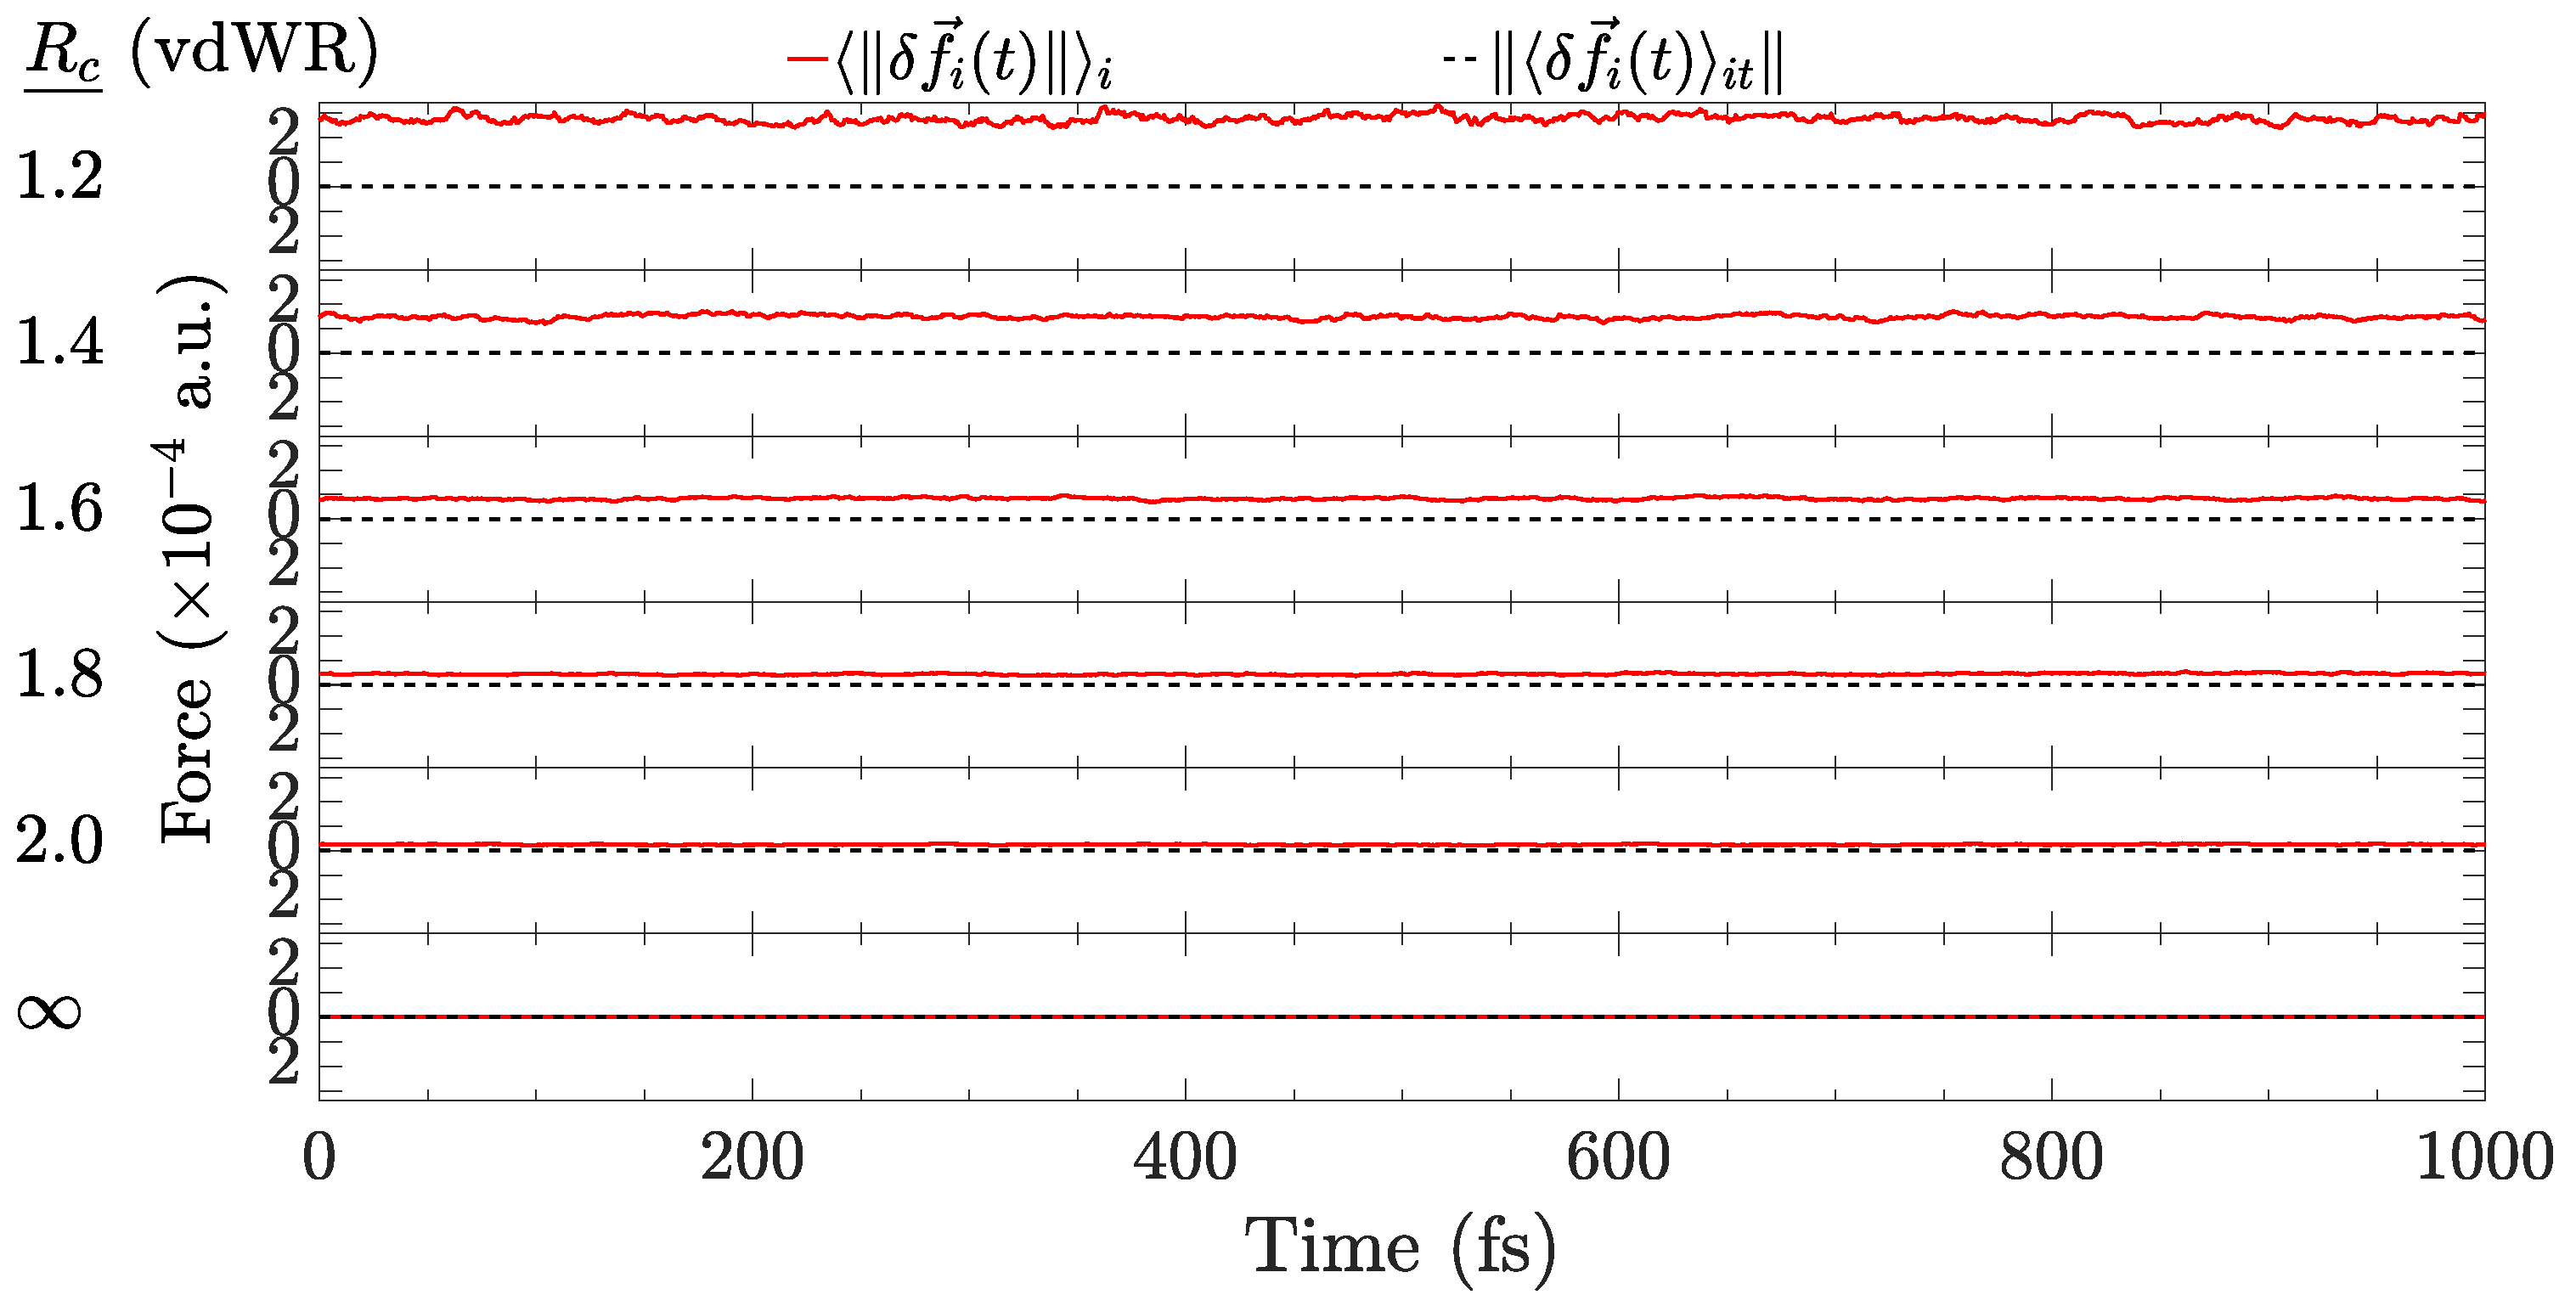
\includegraphics[trim={0cm 0cm 0.1cm 0.1cm},clip,width=8.6cm]{5.eps}
\caption{\label{fig:forcecomp} Dependence of the Euclidean norm of the instantaneous error $\langle \| \delta \vec{f_{i}}(t) \| \rangle_{i}$ (red line) on the ALMO localization radius $R_c$ expressed in units of atomic van der Waals radii. Black line is the magnitude of the time average of the instantaneous error vector. %calculated as the average difference between fully converged Born-Oppenheimer forces and fully converged ALMO DFT forces, averaged over all dimensions and all molecules for each time step. 
Forces are computed with the PBE exchange-correlation functional, TZV2P basis set, and $\epsilon_{\text{SCF}} = 10^{-7}$~a.u. for the configurations from a 30-ps trajectory generated with delocalized AIMD at T=298~K.}
\end{figure}

\bibliography{SI}

\end{document}
